\documentclass[a4paper,10pt]{article}

%%%%%%%%%%%%%%%%%%%%%%%%%%%%%%%%%%%%%%%%%%%%%%%%%%
% Los paquetes permiten ampliar las capacidades de LaTeX.                     %
%%%%%%%%%%%%%%%%%%%%%%%%%%%%%%%%%%%%%%%%%%%%%%%%%%
% Paquete para inclusión de gráficos.
\usepackage{graphicx}

% Paquete para definir la codificación del conjunto de caracteres usado
\usepackage[utf8x]{inputenc}

% Paquete para definir el idioma usado.
\usepackage[spanish]{babel}

% Paquete para introducir codigo de programacion
\usepackage{listings}

 % Para poder introducir otrod PDFs
\usepackage{pdfpages}

% Para inseratar imagenes
\usepackage{graphicx}
\usepackage{subfigure}

% Título principal del documento.
\title{\textbf{Trabajo Practico 0: Infraestructura Basica}}


% Información sobre los autores.
\author{Augusto Arturi (\#97498)\\
\texttt{turitoh@gmail.com}\\
\\
Matias Rozanec (\#97404)\\            \texttt{rozanecm@gmail.com}\\
\\
Agustin Miguel Payaslian (\#96.885)\\            \texttt{payas17@hotmail.com}\\
\\
\normalsize{Grupo Nro. \# - 2do. Cuatrimestre de 2017}\\
\\
\\
\normalsize{66.20 Organización de Computadoras}\\
\normalsize{Facultad de Ingeniería, Universidad de Buenos Aires}\\
}
\date{7/09/2017}


\begin{document}

% Inserta el título.
\maketitle
% Quita el número en la primer página.
\thispagestyle{empty}
% Resumen

\newpage
\begin{abstract}

El trabajo consiste en programar la Criba de Eratostenes,con el objetivo de familiarizarse con las herramientas que utilizaremos a lo largo del curso.
\end{abstract}


\section{Introducción}
Aquí se comenta en forma escueta como está constituido el presente informe, donde  básicamente  se  encuentran  dos  secciones  principales: Desarrollo y Conclusiones.\\
En Desarrollo se encuentran breves comentarios sobre la implementacion del algoritmo como tambien, las corridas de prueba del programa. En la seccion conclusiones se discuten los resultados obtenidos.

\section{Desarrollo}

\subsection{Implementacion}

\subsection{Corridas de prueba}

\section{Conclusiones}

Como hemos visto en los ejercicios anteriores,con los problemas de seguridad que presentan los programas compilados en C, se puede modificar el valor de una variable con el hecho de ingresar un string. Esto no es un problema menor ya que asi como modificamos el valor de una variable, tambien se puede llamar a una funcion dentro del programa o hasta se pueden ingresar instrucciones. Esto puede llegar a generar inconvenientes a la hora de tener un programa con ingreso de usuario y contrasena o cualquier otro en el que se necesite el ingreso de datos, ya que se puede escribir codigo malicioso por las entrada manipulando el programa de la forma deseada.

Una posible solucion a este problema es chequear la cantidad de caracteres que se estan ingresando y cortar la entrada una vez alcanzado el tamano del buffer.

% Apendices
\appendix
\section{Apendice A:Codigo fuente}\label{aped.a}
\section{Apendice B:Enunciado}\label{aped.b}
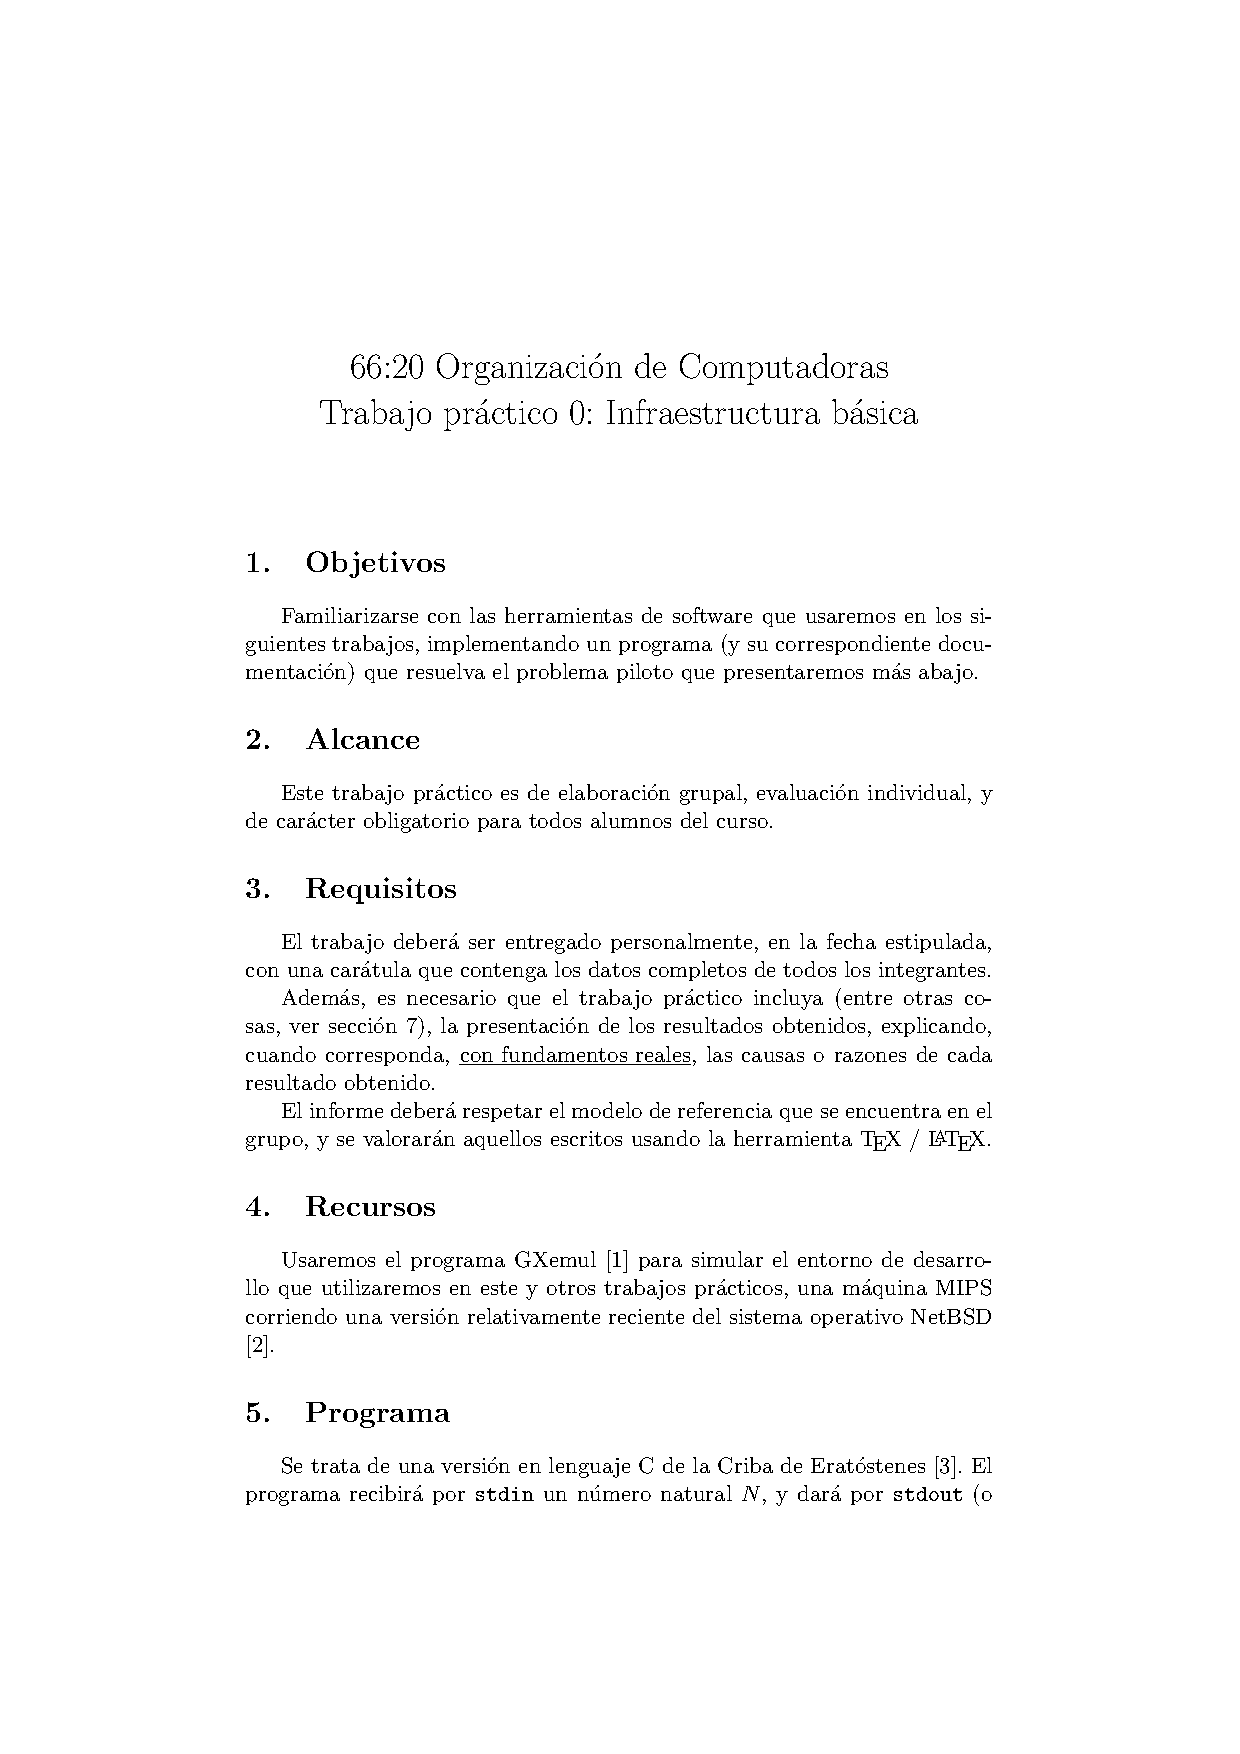
\includepdf[pages=-]{Enunciado.pdf}

\end{document}
